\section{DenseNet}
\subsection{DenseNet là gì}
DenseNet - Dense Convolutional Network (Mạng Tích chập Kết nối Dày đặc) - là một trong những biến thể mở rộng của Resnet và là một kiến trúc mạng,trong đó mỗi lớp được kết nối trực tiếp với mỗi lớp khác nhau theo kiểu chuyển tiếp (trong mỗi khối dense block). Đối với mỗi lớp, các bản đồ đặc trưng (feature map) của tất cả các lớp ở phần trước được coi là các đầu vào riêng biệt và ở đó các bản đồ tính năng lại tiếp tục làm đầu vào cho tất cả các lớp tiếp theo. Cấu trúc mạng này mang lại độ chính xác “state of the art” trên CIFAR. Trên bộ dữ liệu ILSVRC 2012 (ImageNet), DensetNet đạt được độ chính xác tương tự như ResNet, nhưng sử dụng ít hơn một nửa số lượng tham số. DenseNet có cấu trúc gồm các dense block và các transaction layers. Trong kiến trúc CNN truyền thống, nếu có L Layer thì có L connection, trong densenet sẽ có L(L+1)/2 connection\cite{densenetlagi}.

\begin{figure}[H]
	\centering
	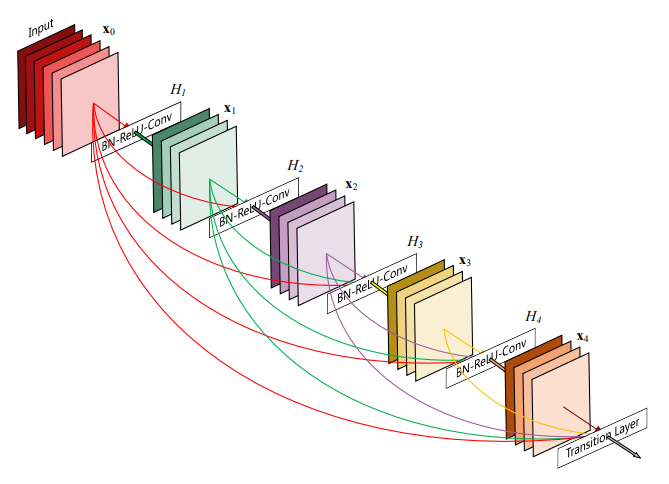
\includegraphics[width=0.8\linewidth]{images/densenet_hl}
	\caption{Kiến trúc DenseNet.}
	\label{fig:kien_truc_densenet}
\end{figure} 

Xét một hình ảnh $x_0$ duy nhất được truyền qua một mạng tích chập. Mạng bao gồm $L$ lớp, mỗi lớp thực hiện một phép biến đổi phi tuyến tính $H_l$(·), trong đó $l$ là chỉ mục các lớp. $H_l$(·) có thể là một hàm tổng hợp của các hoạt động như Batch Normalization (BN), lớp ReLU, lớp Pooling, hoặc lớp Convolution (Conv). DenseNet biểu thị đầu ra của lớp thứ $l$ như là $x_l$.\\
{\bf Kết nối dày đặc - Dense connectivity}
Để cải thiện hơn nữa luồng thông tin giữa các lớp, DenseNet đề xuất một mô hình kết nối mà từ bất kỳ lớp nào cũng có thể kết nối đến tất cả các lớp tiếp theo. Hình \ref{fig:kien_truc_densenet} minh họa bố trí kiến trúc của DenseNet. Dễ dàng nhìn thấy, lớp thứ $l$ nhận được các bản đồ đặc trưng của tất cả các lớp trước đó, $x_0, x_1, x_2, . . . , x_{l-1}),$ làm đầu vào:
\begin{equation}\label{eq:denseconnectivity}
	x_l = H_l([x_0, x_1, . . . , x_{l-1}])
\end{equation}
với $[x_0, x_1, . . . , x{l-1}]$ đề cập đến việc nối các trích chọn đặc trưng được tạo thành trong các lớp $0, 1, ..., {l-1}$. Do khả năng kết nối dày đặc của nó, Gao Huang\cite{densenet} gọi kiến trúc mạng này là Mạng kết nối dày đặc (DenseNet). Để dễ thực hiện, DenseNet nối nhiều đầu vào của $H_l$(·) trong phương trình \ref{eq:denseconnectivity} thành một tensor duy nhất.\\
{\bf Hàm tổng hợp - Composite function}
Ta định nghĩa $H_l$(·) là một hàm tổng hợp của ba hoạt động liên tiếp: Batch Normalization (BN), tiếp theo là một hàm tinh chỉnh các đơn vị tuyến tính (ReLU) và một tích chập 3 × 3 (Conv).\\
{\bf Tầng hợp nhất - Pooling layers}
Thao tác nối được sử dụng trong Phương trình \ref{eq:denseconnectivity} không khả thi khi kích thước của bản đồ đối tượng thay đổi. Tuy nhiên, một phần thiết yếu của mạng tích chập là các lớp lấy mẫu xuống làm thay đổi kích thước của bản đồ đối tượng. Để tạo điều kiện thuận lợi cho việc giảm tần số lấy mẫu trong kiến trúc, DenseNet chia mạng thành nhiều khối dày đặc được kết nối với nhau(hình \ref{fig:densenet_3blk}). DensetNet đề cập đến các lớp giữa các khối là các lớp chuyển tiếp, các lớp này thực hiện tích chập và tổng hợp. Các lớp chuyển tiếp được sử dụng trong các cấu trúc DenseNet bao gồm lớp chuẩn hóa hàng loạt và lớp tích chập 1 × 1, tiếp theo là lớp gộp trung bình 2 × 2.
\begin{figure}[H]
	\centering
	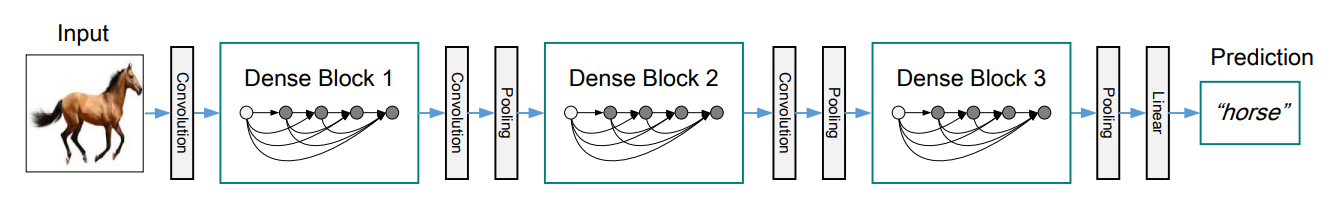
\includegraphics[width=1\linewidth]{images/densenet_3blk}
	\caption{Một DenseNet sâu với ba khối dày đặc.}
	\label{fig:densenet_3blk}
\end{figure}
{\bf Tỉ lệ phát triển - Growth rate}
Nếu mỗi hàm $H_l$ tạo ra $k$ bản đồ đặc trưng, thì lớp thứ $l$ có $k_0 + k{l-1}$ bản đồ đặc trưng đầu vào, trong đó $k_0$ là số kênh trong lớp đầu vào. Một điểm khác biệt quan trọng giữa DenseNet và các kiến trúc mạng trước đó là DenseNet có thể có các lớp rất hẹp, ví dụ: $k = 12$. Ta gọi siêu tham số $k$ là tỉ lệ phát triển của mạng. Tỉ lệ phát triển quy định lượng thông tin mới mà mỗi lớp đóng góp vào trạng thái toàn cục. Trạng thái toàn cục, sau khi được lưu trữ, có thể được truy cập từ mọi nơi trong mạng mà không cần phải sao chép nó từ lớp này sang lớp khác - không giống như trong các kiến trúc mạng truyền thống.\\
{\bf Các lớp nút cổ chai - Bottleneck layers}
Mặc dù mỗi lớp chỉ tạo ra $k$ bản đồ đặc trưng đầu ra, nhưng nó thường có nhiều đầu vào hơn. Người ta lưu ý rằng tích chập 1 × 1 có thể được đưa vào làm lớp nút cổ chai trước mỗi tích chập 3 × 3 để giảm số lượng bản đồ đặc trưng đầu vào và từ đó để cải thiện hiệu quả tính toán. Thiết kế này đặc biệt hiệu quả đối với DenseNet.\\
{\bf Độ nén - Compression}
Để cải thiện hơn nữa độ nhỏ gọn của mô hình, chúng ta có thể giảm số lượng bản đồ đặc trưng ở các lớp chuyển tiếp. Nếu một khối dày đặc chứa $m$ bản đồ đặc trưng, để lớp chuyển tiếp sau tạo ra $\theta m$ bản đồ đặc trưng đầu ra, trong đó $0 < \theta \leq 1$ được gọi là hệ số nén. Khi $\theta = 1$, số lượng bản đồ đối tượng trên các lớp chuyển tiếp không thay đổi.

\subsection{Kiến trúc của DenseNet}
Từ hình \ref{fig:densenet_3blk}, có thể nhận thấy rằng DenseNets được chia thành nhiều khối dày đặc DenseBlock. Các kiến trúc khác nhau của DenseNets đã được tóm tắt trong bài báo "Densely Connected Convolutional Networks"\cite{densenet}. 

Mỗi kiến trúc bao gồm bốn DenseBlock với số lượng lớp khác nhau. Ví dụ, DenseNet-121 có [6,12,24,16] lớp trong bốn khối dày đặc trong khi DenseNet-169 có [6, 12, 32, 32] lớp. Chúng ta có thể thấy rằng phần đầu tiên của kiến trúc DenseNet bao gồm Lớp chuyển đổi 2 bước 7x7, tiếp theo là lớp MaxPooling 3x3 bước-2. Và khối dày đặc thứ tư được theo sau bởi một Lớp phân loại chấp nhận các bản đồ đặc trưng của tất cả các lớp của mạng để thực hiện phân loại. 

Ngoài ra, các phép toán tích chập bên trong mỗi kiến trúc là các lớp Cổ chai. Điều này có nghĩa là Conv 1x1 làm giảm số lượng kênh trong đầu vào và Conv 3x3 thực hiện hoạt động tích chập trên phiên bản đã biến đổi của đầu vào với số lượng kênh giảm hơn so với đầu vào.
\begin{figure}[H]
	\centering
	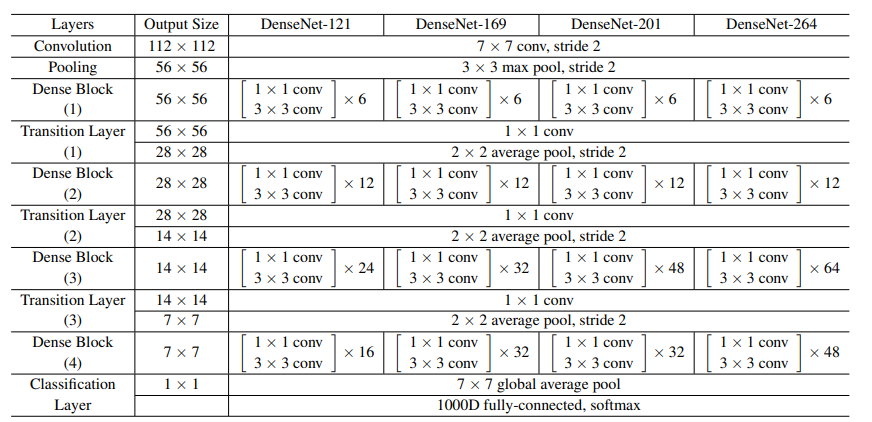
\includegraphics[width=1\linewidth]{images/densenet_archtectures_for_imagenet}
	\caption{Các kiến trúc DenseNet.}
	\label{fig:densenet_archtectures_for_imagenet}
\end{figure}

\subsection{Cài đặt DenseNet}
\begin{lstlisting}[language=Python]
def DenseNet(input_shape=(512, 512, 1),nb_dense_block=4, growth_rate=32, nb_filter=64, reduction=0.0, dropout_rate=0.0, weight_decay=1e-4, classes=1000, weights_path=None):

	eps = 1.1e-5
	
	compression = 1.0 - reduction
	
	global concat_axis
	concat_axis = 3
	img_input = Input(shape=input_shape, name='data')
	
	# From architecture for ImageNet (Table 1 in the paper)
	nb_filter = 64
	nb_layers = [6,12,24,16] # For DenseNet-121
	
	# Initial convolution
	x = ZeroPadding2D((3, 3), name='conv1_zeropadding')(img_input)
	x = Convolution2D(nb_filter, 7, 7, subsample=(2, 2), name='conv1', bias=False)(x)
	x = batch_normalization(epsilon=eps, axis=concat_axis, name='conv1_bn')(x)
	x = Activation('relu', name='relu1')(x)
	x = ZeroPadding2D((1, 1), name='pool1_zeropadding')(x)
	x = MaxPooling2D((3, 3), strides=(2, 2), name='pool1')(x)
	
	# Add dense blocks
	for block_idx in range(nb_dense_block - 1):
	stage = block_idx+2
	x, nb_filter = dense_block(x, stage, nb_layers[block_idx], nb_filter, growth_rate, dropout_rate=dropout_rate, weight_decay=weight_decay)
	
	# Add transition_block
	x = transition_block(x, stage, nb_filter, compression=compression, dropout_rate=dropout_rate, weight_decay=weight_decay)
	nb_filter = int(nb_filter * compression)
	
	final_stage = stage + 1
	x, nb_filter = dense_block(x, final_stage, nb_layers[-1], nb_filter, growth_rate, dropout_rate=dropout_rate, weight_decay=weight_decay)
	
	x = batch_normalization(epsilon=eps, axis=concat_axis, name='conv'+str(final_stage)+'_blk_bn')(x)
	x = Activation('relu', name='relu'+str(final_stage)+'_blk')(x)
	x = GlobalAveragePooling2D(name='pool'+str(final_stage))(x)
	
	x = Dense(classes, name='fc6')(x)
	x = Activation('softmax', name='prob')(x)
	
	model = Model(img_input, x, name='densenet')
	
	if weights_path is not None:
	model.load_weights(weights_path)
	
	return model
	
	
def conv_block(x, stage, branch, nb_filter, dropout_rate=None, weight_decay=1e-4):
	eps = 1.1e-5
	conv_name_base = 'conv' + str(stage) + '_' + str(branch)
	relu_name_base = 'relu' + str(stage) + '_' + str(branch)
	
	# 1x1 Convolution (Bottleneck layer)
	inter_channel = nb_filter * 4  
	x = batch_normalization(epsilon=eps, axis=concat_axis, name=conv_name_base+'_x1_bn')(x)
	x = Activation('relu', name=relu_name_base+'_x1')(x)
	x = Convolution2D(inter_channel, 1, 1, name=conv_name_base+'_x1', bias=False)(x)
	
	if dropout_rate:
	x = Dropout(dropout_rate)(x)
	
	# 3x3 Convolution
	x = batch_normalization(epsilon=eps, axis=concat_axis, name=conv_name_base+'_x2_bn')(x)
	x = Activation('relu', name=relu_name_base+'_x2')(x)
	x = ZeroPadding2D((1, 1), name=conv_name_base+'_x2_zeropadding')(x)
	x = Convolution2D(nb_filter, 3, 3, name=conv_name_base+'_x2', bias=False)(x)
	
	if dropout_rate:
	x = Dropout(dropout_rate)(x)
	
	return x
	
	
def transition_block(x, stage, nb_filter, compression=1.0, dropout_rate=None, weight_decay=1E-4):
	eps = 1.1e-5
	conv_name_base = 'conv' + str(stage) + '_blk'
	relu_name_base = 'relu' + str(stage) + '_blk'
	pool_name_base = 'pool' + str(stage) 
	
	x = batch_normalization(epsilon=eps, axis=concat_axis, name=conv_name_base+'_bn')(x)
	x = Activation('relu', name=relu_name_base)(x)
	x = Convolution2D(int(nb_filter * compression), 1, 1, name=conv_name_base, bias=False)(x)
	
	if dropout_rate:
	x = Dropout(dropout_rate)(x)
	
	x = AveragePooling2D((2, 2), strides=(2, 2), name=pool_name_base)(x)
	
	return x
	
	
def dense_block(x, stage, nb_layers, nb_filter, growth_rate, dropout_rate=None, weight_decay=1e-4, grow_nb_filters=True):
	concat_feat = x
	
	for i in range(nb_layers):
	branch = i+1
	x = conv_block(concat_feat, stage, branch, growth_rate, dropout_rate, weight_decay)
	concat_feat = merging([concat_feat, x], mode='concat', concat_axis=concat_axis, name='concat_'+str(stage)+'_'+str(branch))
	
	if grow_nb_filters:
	nb_filter += growth_rate
	
	return concat_feat, nb_filter
\end{lstlisting}

\subsection{Áp dụng DenseNet vào bài toán của luận văn}
